\chapter[Uitvoering]{Uitvoering}
\label{chap_uitvoering}

\section{Opzetten van een lokale webserver}
Op aanraden van \'{e}\'{e}n van de collega's zetten we een Tomcat Apache server op via Eclipse om onze website op te draaien. Via de volgende links kan je deze software downloaden:
\begin{itemize}
\item Apache Tomcat v7.0: \url{http://tomcat.apache.org/download-70.cgi}
\item Eclipse IDE for Java EE Developer:  \url{https://www.eclipse.org/downloads/}
\end{itemize} 
Start Eclipse op en maak een nieuwe workspace aan. Klik met je rechtermuisknop onderaan in de Servers tab. Klik dan op New \textgreater Server en selecteer de volgende instellingen:
\begin{center}
  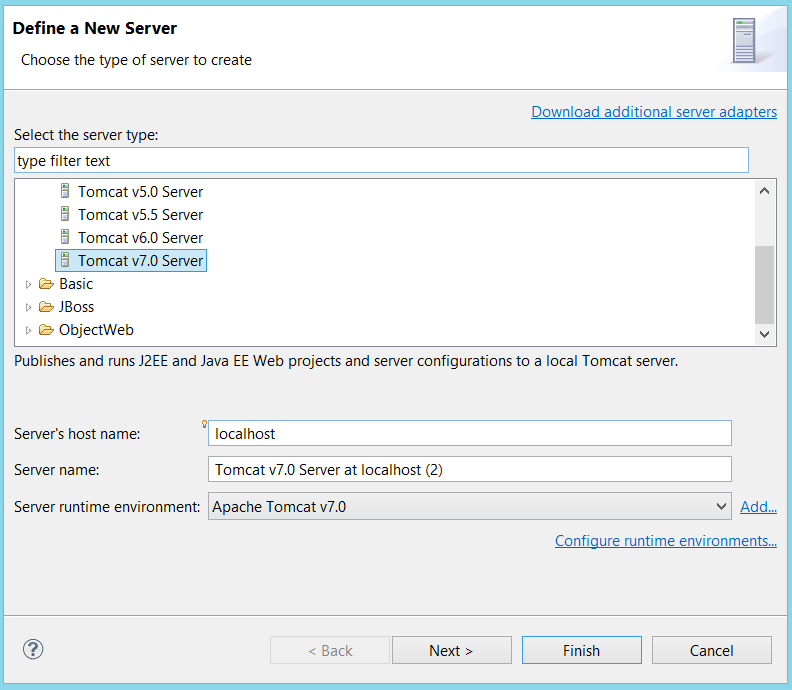
\includegraphics[width=0.95\textwidth]{figures/chap2/eclipse1.png}
  \captionof{figure}[Screenshot Eclipse server settings]{Screenshot Eclipse server settings
  \label{fig_eclipse1}}
\end{center}

Klik Next en klik Finish. De server zal wanneer hij gestart is de files uploaden naar localhost:8080. Deze files zitten in de Tomcat folder die je eerder hebt geinstalleerd met het volgende pad:
\begin{itemize}
\item C:\textbackslash Users\textbackslash Crauwels Dries\textbackslash Documents\textbackslash Tomcat\textbackslash webapps\textbackslash ROOT
\end{itemize}
Hierin komt dan ook onze folder die onze website zal bevatten.
Om de server te starten selecteren we ze in Eclipse in de servers tab en drukken we op start.
Als alles werkt kunnen we naar http://localhost:8080/ surfen en zien we de homepage van Tomcat:
\begin{center}
  
\includegraphics[width=0.95\textwidth]{figures/chap2/tomcathomepage.png}
  \captionof{figure}[Screenshot Tomcat Homepage]{Screenshot Tomcat Homepage
  \label{fig_tomcat1}}
\end{center}

De link naar onze eigen files wordt dan: http://localhost:8080/MyFolder/index.html \newline
Nu kunnen we van start gaan met de structuur van de applicatie en het schrijven van onze html paginas.

\section{Algemene mappenstructuur}

De code zal opgesplitst zijn in 3 typen bestanden: .HTML bestanden, .CSS bestanden en .JS bestanden. De HTML bestanden zullen de basis HTML bevatten voor onze website. Het is het skelet van de structuur en bevat de inhoud van de pagina. Het stijlen van de pagina gebeurt in CSS en zoveel mogelijk code zal in aparte .JS bestanden staan. Zoals onze eigen library met alle D3 code en externe plugins.

Wanneer we refereren naar \'{e}\'{e}n van deze bestanden vanuit een HTML pagina dan moeten we het pad opgeven dat vertrekt vanuit de plaats waar de HTML pagina zelf bevindt. Met andere woorden als index.html in onze MyFolder zit en daarin zit een JS map met library.js, dan moet de index pagina het /JS/library.js pad gebruiken om hieraan te kunnen. Het is dan ook voor de hand liggend dat we een mappenstructuur handhaven die er als volgt uitziet:

Alle HTML paginas zitten in de website folder. CSS in de CSS folder en de Javascript bestanden in JS. Voorts is er nog een map voor figuren, data en fonts.
\begin{itemize}
\item D3-Chart-Wizard
	\begin{itemize}
	\item home.html
	\item barchart.html
	\item linechart.html
	\item donutchart.html
	\item areachart.html
	\item infographic.html
	\item js
		\begin{itemize}
		\item jquery-ui.js
		\item chartwizard.js
		\item ...
		\end{itemize}
	\item css
		\begin{itemize}
		\item jquery-ui.css
		\item charts.css
		\item menu.css
		\item infographic.css
		\item ...
		\end{itemize}
	\item data
	\item fonts
	\item images
	\end{itemize}
\end{itemize}

\section{Algemene code-architectuur en opmaak}

Goede code schrijven is belangrijk. Zoals Mr. Dams altijd zegt: schrijf geen dubbele code, wees consistent, begrijp wat je schrijft en hoe minder code nodig om het te doen laten werken hoe beter. Elke soort code zal een andere opmaak en structuur hebben naargelang de mogelijkheden van de taal. 

\textbf{HTML}

HTML is geen programmeertaal maar een opmaaktaal. Dit wil echter niet zeggen dat we geen structuur moeten handhaven en niet aan een aantal afspraken moeten houden. In de HTML paginas is het belangrijkste dat de ID attributen uniek zijn en dat ze een logische naam hebben. Een logische naam moet kort zijn maar uniek en verwijzen naar welk element het inzit. Stel dat het een ID is van een div waarin meerdere divs zitten dan kunnen we dit een wrapper of container noemen. Bijvoorbeeld \textless div id="svg-container"\textgreater  is de div waarin de SVG elementen zitten. Verder zullen de class names in alle tags gebruikt worden voor de opmaak van het element. Class attributen mogen meerdere keren voorkomen zodanig dat elk element met dezelfde class name dezelfde stijling krijgt en kan een javascript functie alle elementen aanroepen met deze class name. 

De opmaak van de code kan je makkelijk doen door je code op een online source-formatter te kopieren. Zo krijgen alle lijnen de juiste inspringing en krijg je veel beter overzicht van je code indien je slim genoeg bent om hier geen tijd in te steken of het gewoon niet goed kan. Dreamweaver kan dit ook maar minder goed.

\url{http://jsbeautifier.org/}

\textbf{CSS}

De CSS bestanden hebben geen specifieke opmaak aangezien CSS niets speciaal is wat code betreft.

\textbf{JavaScript}

Het meeste van de JavaScript code zal in onze eigen library staan. Deze library is een namespace waarin we classes en functions kunnen steken die we kunnen aanroepen vanuit de HTML pagina als de library geinclude wordt. 
variabele charts is de namespace en elke functie die volgt na een "." zit in deze namespace. Als we dit .js bestand includen in onze HTML pagina kunnen we deze functies aanroepen met "charts.class1.subclass1.functie()" bijvoorbeeld.

De opmaak ziet er zo uit: 

\lstset{numbers=left, stepnumber=1, basicstyle=\footnotesize, frame=none, xleftmargin=.3in}
\begin{lstlisting}
// JavaScript Library Document
// Library.js

var charts = charts || {};

(function () {
        //General variables
        var margin = {
                top: 0,
                right: 0,
                bottom: 76,
                left: 76
        };


        var svgWidth = 1080 - margin.left - margin.right,
                svgHeight = 400 - margin.top - margin.bottom;

        var HDsvgWidth = 1920,
                HDsvgHeight = 1080;
                
        charts.infographic = function (type) {
                 var graphicType;
                 
                 graphicType = type;
                 switch(graphicType){
                     case "DNA-graphic":
                     
                     charts.infographic.DNAgraphic = function (divclass) {
                         
                           
\end{lstlisting}

Elke HTML pagina zal zijn eigen code hebben maar er kunnen meerdere paginas zijn die dezelfde CSS gebruiken en libraries. Zo is er \'{e}\'{e}n CSS die de twee navigatie menus bovenaan stijlt, een CSS voor de infographic wizard en \'{e}\'{e}n voor alle chart wizards. 

Alle JavaScript code die we in de HTML pagina gebruiken verdelen we onder in 4 categorie\"{e}n: initialisations, jQuery UI, D3  en JavaScript. Al deze code zetten we onderaan in de \textless body\textgreater  om de pagina sneller te doen laden.

In initialisations zetten we alles wat in de document.ready functie moet.

\begin{center}
  
\includegraphics[width=0.95\textwidth]{figures/chap2/initialisations.png}
\end{center}

jQuery heeft voor het aanroepen van al zijn UI elementen methodes nodig. Deze komen onder de jQuery UI comment.

\begin{center}
  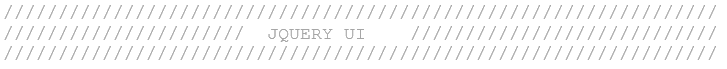
\includegraphics[width=0.95\textwidth]{figures/chap2/jqueryui.png}
\end{center}


Onder D3 komt alle nodige D3 code die te klein is om in de library te steken.

\begin{center}
  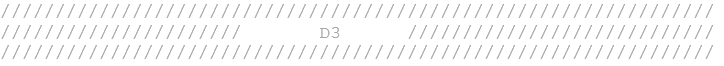
\includegraphics[width=0.95\textwidth]{figures/chap2/d3.png}
\end{center}

Al de JavaScript die niet in de vorige categorieen thuishoort zetten we hier.

\begin{center}
  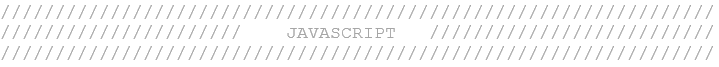
\includegraphics[width=0.95\textwidth]{figures/chap2/javascript.png}
\end{center}

Indien er globale variabelen moeten zijn komen die bovenaan onder elke categorie te staan.

\section{Web IDE}
Als je iets gaat ontwikkelen voor het web dat zowel CSS, HTML als JavaScript bevat, bestaat er geen standaard ontwikkelomgeving. Deze applicatie is geschreven met behulp van Dreamweaver CS6[1] van Adobe dat nog een degelijke ondersteuning aanbiedt. De nieuwste Visual Studio[2] blijkt ook goed mee te vallen maar na wat onderzoek te hebben gedaan achteraf is gebleken dat WebStorm[3] van JetBrains de beste IDE is voor web development. JetBrains is trouwens dezelfde producent van ReSharper voor Visual Studio. Helaas is geen enkel van deze software gratis.

\begin{itemize}
 \item $[1]$: \url{http://www.adobe.com/be_nl/products/dreamweaver/features.html}
 \item $[2]$: \url{http://www.visualstudio.com/explore/application-development-vs#Scenario2_1}
 \item $[3]$: \url{http://www.jetbrains.com/webstorm}
\end{itemize}

Wat wel zeer handig is in Dreamweaver is de Find and Replace feature. Deze is simpel maar krachtig. De andere web IDE's zullen dit zeker ook wel hebben. Hiermee kan je verschillende tags selecteren en bijvoorbeeld bepaalde attributen met een bepaalde waarde veranderen. Zo hoef je ze niet \'e\'en voor \'e\'en alles aan te passen.

\begin{center}
  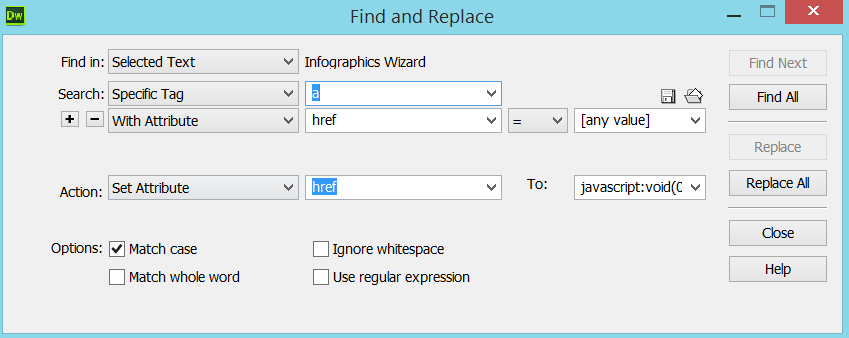
\includegraphics[width=0.95\textwidth]{figures/chap2/dreamweaver.png}
\end{center}

\section{Git en Versiecontrole}
Bij Inventive Designers maken ze gebruik van Stash van Atlassian. Een manier om beter gebruik te maken van Git met servers, taakverdeling en meerdere gebruikers.

\textit{Git repository management your way
On-premises source code management for Git that's secure, fast, and enterprise grade. Create and manage repositories, set up fine-grained permissions, and collaborate on code - all with the flexibility of your servers.}

Source: Stash - \url{https://www.atlassian.com}

\textbf{Git GUI}

Om makkelijker overweg te kunnen met Git zonder commandline maken we gebruik van SourceTree. Dit is een grafishe interface waarmee we eenvoudig de repository kunnen binnenhalen van Stash en er een lokale map van maken. Hierin steken we dan de map met onze volledige website in. We voeren dan een commit en push uit als we deze willen uploaden naar Stash na een grondige verandering. Bij elke commit voegen we commentaar bij met wat er precies veranderd en toegevoegd is.

\begin{center}
  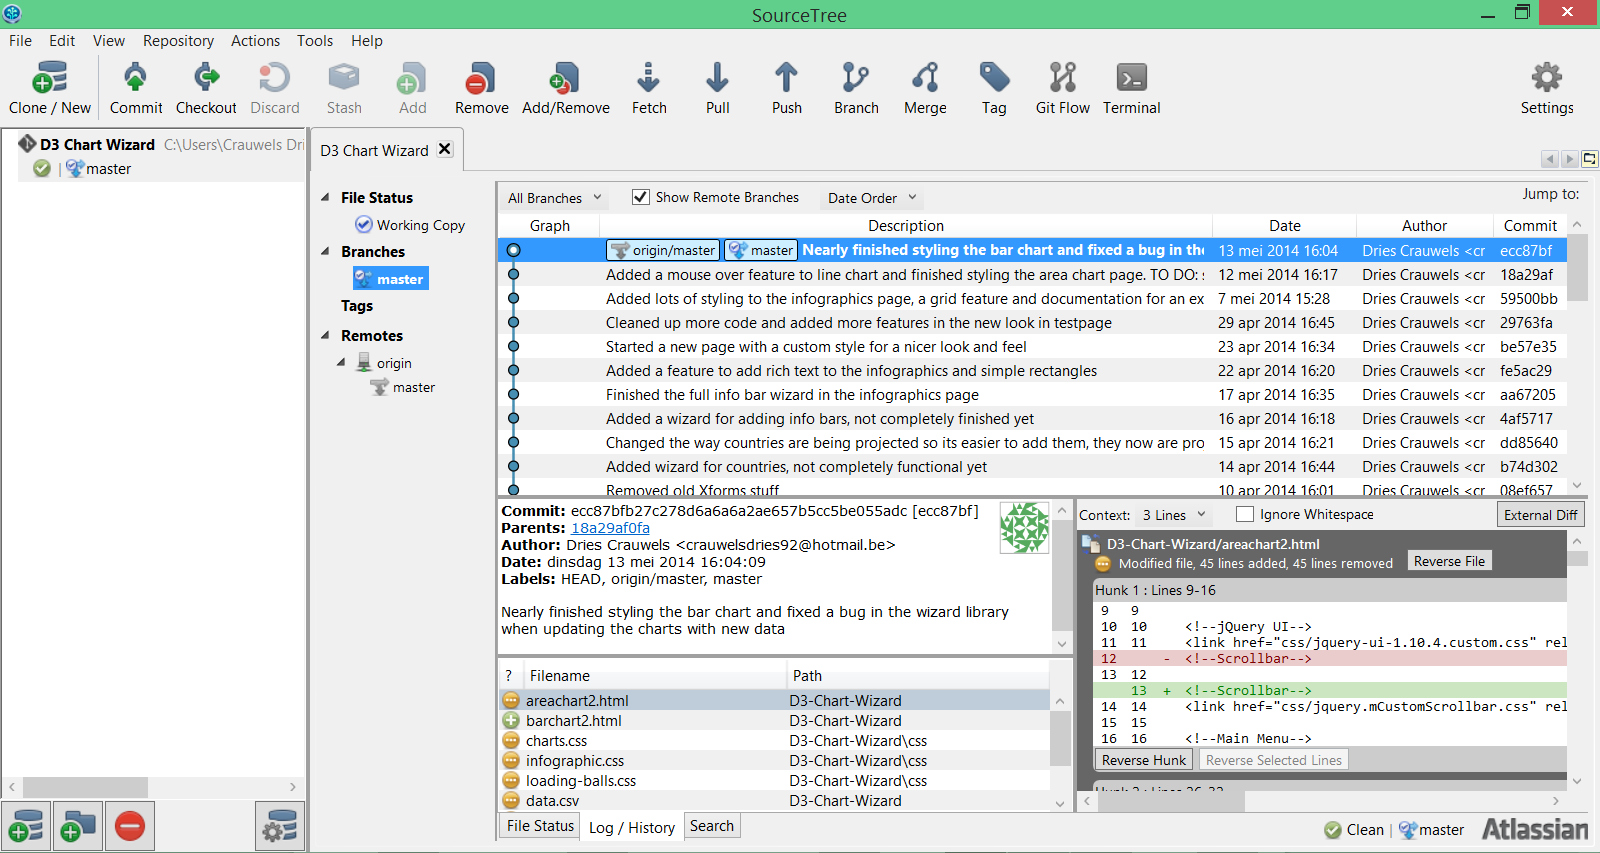
\includegraphics[width=0.95\textwidth]{figures/chap2/sourcetree.png}
  \captionof{figure}[Screenshot SourceTree]{Screenshot SourceTree
  \label{fig_sourcetree}}
\end{center}

\section{SVG en D3}
Scalable Vector Graphics(SVG) zijn HTML elementen om twee-dimensionale figuren weer te geven op het web. Deze elementen worden geschreven in een XML format net zoals ander gewone HTML elementen. Omdat deze elementen vectorieel zijn, is er geen kwaliteitsverlies bij het inzoomen of vergroten en verkleinen. Er is mogelijkheid tot animatie met SVG elementen en je kan ze stijlen met CSS.

\textbf{Voorbeeld van een afgeronde rechthoek met SVG:}

\begin{center}
  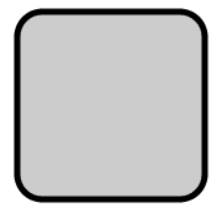
\includegraphics[]{figures/chap2/SVGrectangle.png}
\end{center}

\begin{lstlisting}
<svg width="400" height="180">
  <rect x="50" y="20" rx="20" ry="20" width="150" height="150"
  style="fill:#CCC;stroke:black;stroke-width:5;" />
</svg>
\end{lstlisting}

\textbf{Fiddle: }\url{http://jsfiddle.net/4FSgJ/}

D3(Data Driven Documents) bindt arbitraire data aan een Document Object Model(DOM) en transformeert deze naar het document op een Data-Driven manier. Met andere woorden je kan eender welk HTML element invoegen waarvan de eigenschappen afkomstig zijn uit een dataset zoals een array van objecten. D3 is een JavaScript library en is volledig mee geinteregeerd met de HTML 5 CSS 3 en SVG standaarden.

\textbf{Voorbeeld van een afgeronde rechthoek met D3:}

\begin{center}
  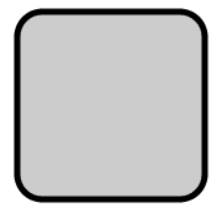
\includegraphics[]{figures/chap2/SVGrectangle.png}
\end{center}

\begin{lstlisting}
<div class="container"></div>
var svg = d3.select(".container")
            .append("svg")
            .attr("width",400)
            .attr("height",180);

svg.append("rect")
        .attr("x",50)
        .attr("y",20)
        .attr("rx",20)
        .attr("ry",20)
        .attr("width",150)
        .attr("height",150)
        .style({"fill":"#CCC",
                "stroke":"black",
                "stroke-width":5});
\end{lstlisting}

\textbf{Fiddle: }\url{http://jsfiddle.net/aZT7c/}

Zoals je kan zien krijgen we twee identieke figuren. Echter de code om deze te genereren met D3 is veel te veel voor wat je krijgt. D3 wordt pas interessant wanneer we dit vierkant gaan visualiseren aan de hand van data en de gebruiker de mogelijkheid geven om dit allemaal zelf te doen. Het eerste vierkant is dan ook "hard-coded" zoals dat heet en is niet dymanisch. Voor een wizard moet alles dynamisch opgebouwd zijn en mag niets vast staan. Elk element en attribuut moet aangepast, toevoegd, of verwijderd kunnen worden.

\textbf{Een complexer voorbeeld van wat D3 kan:}
\begin{center}
  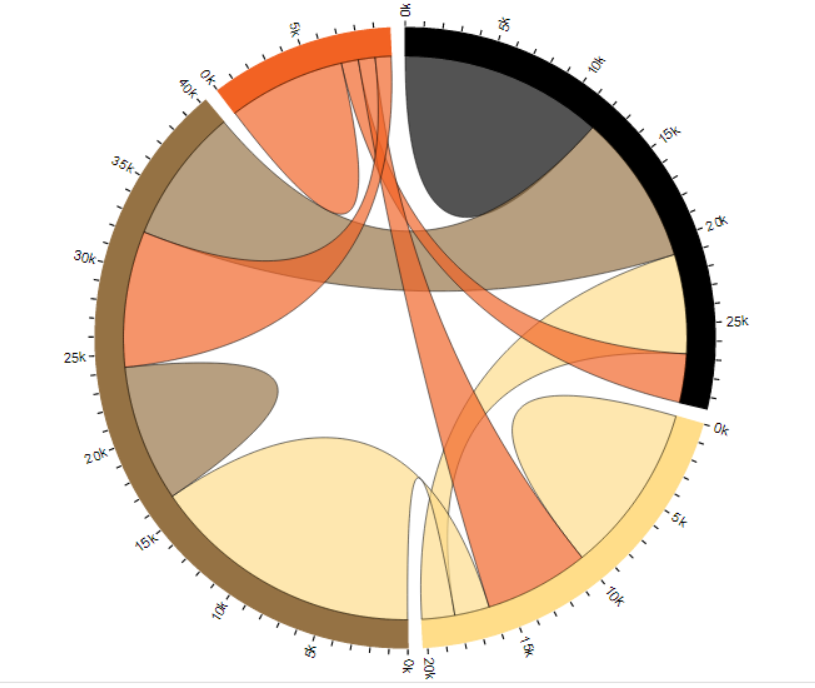
\includegraphics[]{figures/chap2/chorddiagram.png}
\end{center}
\textbf{Voorbeelden met animaties}

\url{http://bl.ocks.org/mbostock/10685278}

\url{http://bl.ocks.org/mbostock/10571478}



\section{Debugging}
Er is niets zo simpel als debuggen wanneer je code schrijft voor het web. Je moet niet wachten om je code te compilen, je slaat je HTML pagina gewoon op en refresht de pagina. Het is de browser zelf die de code zal compilen. Als er dan errors zijn kan je die in de debugger van je browser zien. Deze krijg je te zien als je ergens op de pagina met je rechtermuisknop klikt en "Element inspecteren" selecteert. De meeste browsers hebben een soortgelijke debugging interface. In deze opdracht is altijd Google Chrome gebruikt die er als volgt uitziet:

\begin{center}
  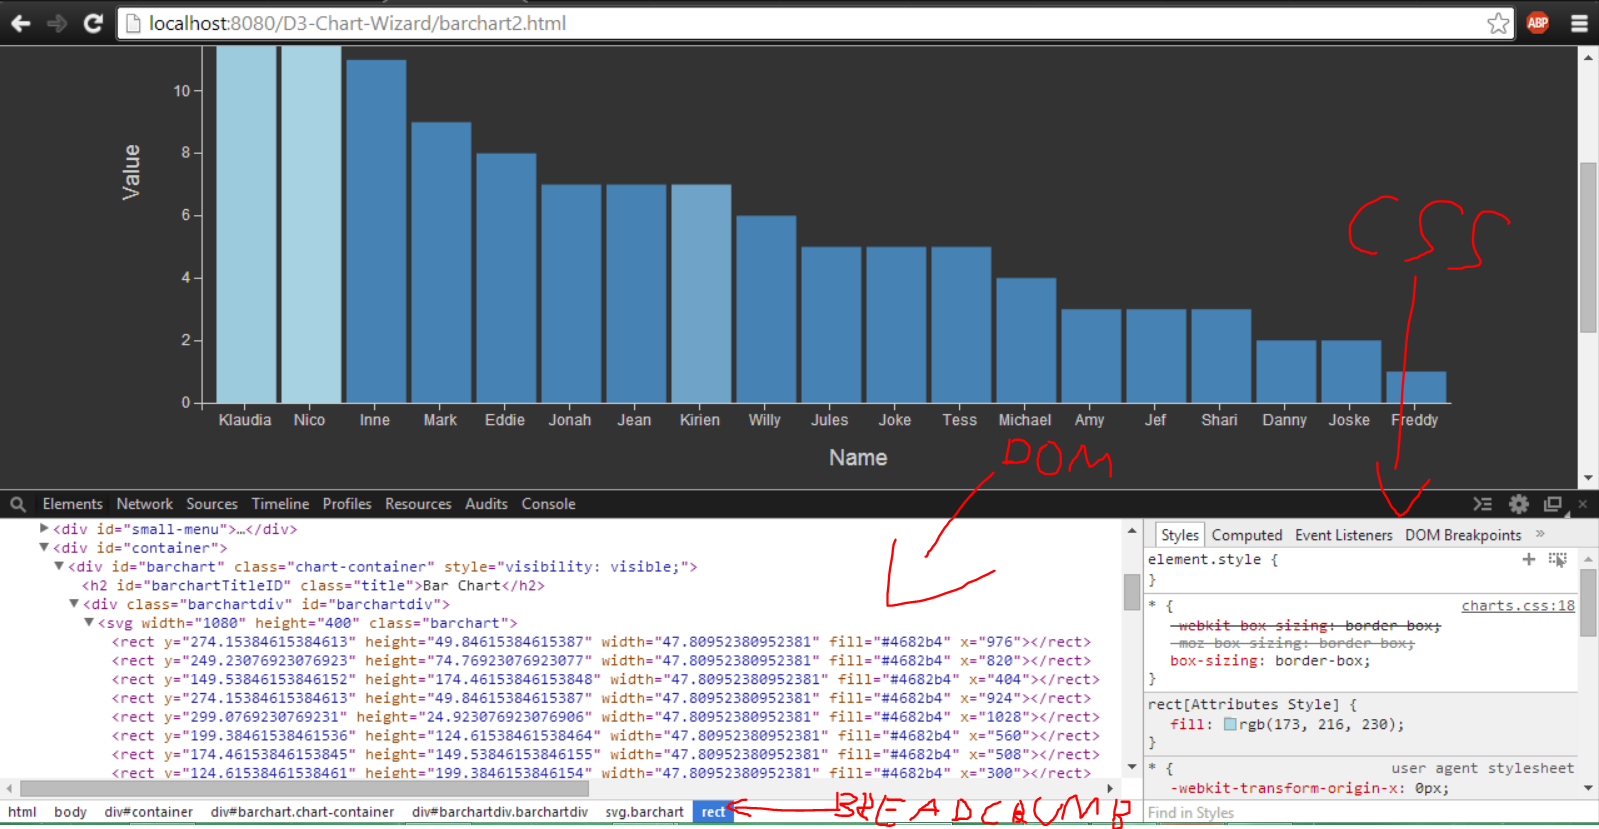
\includegraphics[width=0.95\textwidth]{figures/chap2/chromedebugger.png}
  \captionof{figure}[Screenshot Chrome Debugging Interface]{Screenshot Chrome Debugging Interface
  \label{fig_sourcetree}}
\end{center}

Zoals is aangeduid op de screenshot hebben we links onderaan in onze browser de DOM inspector die alle elementen en hun attributen weergeeft. Als we met onze muis over een element gaan wordt deze geselecteerd in de browser en weten we precies welk element het is. Daaronder zien we ook in welke andere tags het element genest zit. Dit heet een breadcrumb-trail. Ten slotte zien we ook de CSS rechts van het geselecteerde element. We zien welke CSS eigenschappen dit element allemaal krijgt en van waar ze komen.

Indien we met externe JavaScript bestanden werken kunnen we deze zien in de "Sources" tab in de debugger. Hierin kunnen we ook break-points zetten waar de browser zal pauzeren bij het refreshen van de pagina als het break-point eenmalig is of wanneer we op deze plaats in de code zitten bij het uitvoeren van een handeling. Net zoals eender welke andere debugger.

\begin{center}
  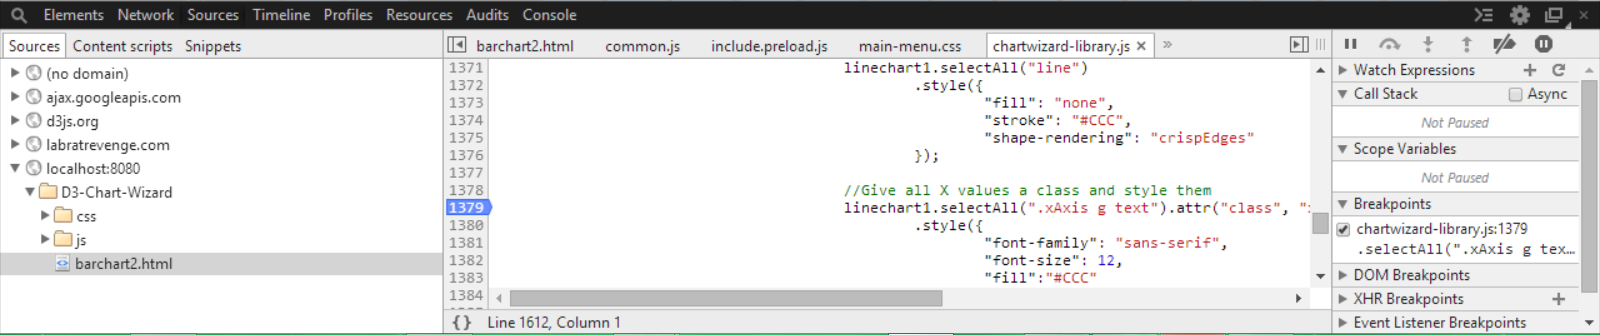
\includegraphics[width=0.95\textwidth]{figures/chap2/sourcestab.png}
  \captionof{figure}[Screenshot Chrome Debugging Interface: Sources]{Screenshot Chrome Debugging Interface: Sources
\label{fig_sourcetree}}
\end{center} 

We kunnen zelfs live onze code testen door de HTML van de pagina aan te passen in de debugger. Je moet deze niet refreshen, dat is de kracht van HTML. Geen event handlers of iets dergelijks. Je verandert gewoon een attribuut of voegt iets toe en deze verandering zal direct te zien zijn op de pagina.

\section{Hulpbronnen}

\textbf{W3 Schools}
\url{http://www.w3schools.com/default.asp}

\textbf{Stackoverflow}
\url{http://stackoverflow.com}

\textbf{D3 Wiki, voorbeelden en API}
\url{https://github.com/mbostock/d3/wiki}

\textbf{Ebook Interactive Data Visualization for the Web}
\url{http://chimera.labs.oreilly.com/books/1230000000345/pr01.html}

\section{Homepage}

Op de homepage van de website zal je meteen alle wizards te zien krijgen. Zowel de vier basic chart wizards als die voor de infographics. Om de pagina op te vullen en om later uit te breiden zijn er ook links toegevoegd voor andere basic charts. Maar deze links staan uit omdat die wizards nooit zijn klaar geraakt.

Bovenaan staat het navigatie-menu dat volledig is opgemaakt uit eigen CSS. Dit menu wordt in de andere paginas ook weergegeven. Het goede aan eigen CSS en minder libraries te gebruiken is dat er dan minder HTTP "gets" moeten worden uitgevoerd en dit doet de pagina veel sneller laden. De CSS voor het navigatie-menu staat in een aparte CSS file genaamd: "main-menu.css".

De blokken waarin elke link naar de wizard staan zijn dynamisch opgebouwd met behulp van de Masonry.js library. Deze library zorgt ervoor dat \textless div\textgreater  elementen worden opgestapeld zoals een bakstenen muur. Het plaatst ze op een zo goed mogelijke manier zodanig dat er zo min mogelijk plaats wordt overgelaten. Masonry kan nog veel meer dan dit maar die functionaliteiten hebben we niet nodig.


\textbf{Voorbeeld van hoe Masonry elementen kan stapelen:}

\begin{center}
  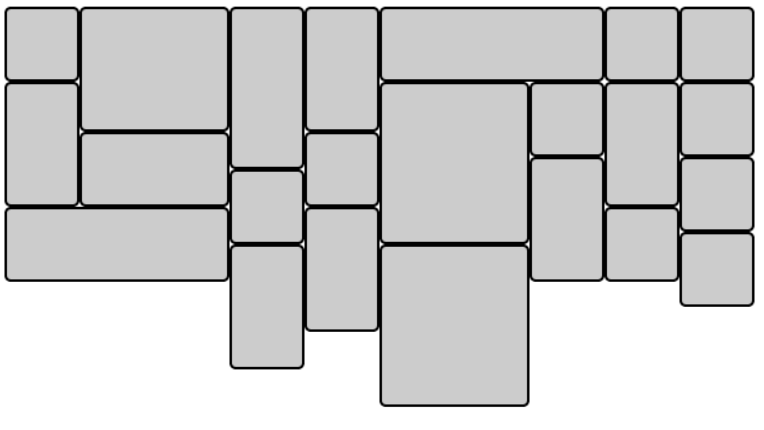
\includegraphics[]{figures/chap2/masonry.png}
\end{center}

\section{Basic Chart Wizards}

Elke basic chart wizard is opgemaakt met dezelfde structuur. Zowel de interface als de code.
Bovenaan staat het algemene navigatie menu. Net daaronder staan de knoppen met alle opties om de chart te bewerken. Elke knop opent een extra dialoogvenster waarin de nodige functies staan. Je kan deze slepen over het scherm zodat je de verandering op de chart direct kan zien. Zoals eerder vermeld zal de belangrijkste code in onze eigen javascript library staan. Dit is de D3 code om de chart te genereren.

De code voor elke chart wizard is zeer analoog. Dit is zowel toevallig als met opzet. Toevallig omdat de charts sterk op elkaar lijken wiskundig gezien(voor elke X waarde steeds maximum \'e\'en Y waarde) en omdat goede code hergebruikt kan worden. Daarom zullen we ook maar \'e\'en chart wizard volledig uitleggen de andere drie zullen in het kort worden toegelicht. Voor de volledige code verwijs ik u naar de bestanden zelf.

\subsection{Area Chart}

Een area chart geeft data weer in de vorm van een opgevuld gebied met X en Y coordinaten. Wiskundig is hier niets speciaal aan. Maar we kunnen dit gebied wel manipuleren. D3 heeft ingebouwde functies om dit te doen. Er zijn verschillende interpolatie mogelijkheden. Om bijvoorbeeld de grafiek af te vlakken kunnen we de Basis-Interpolatie toepassen. De wiskunde hierachter en de kennis om dit in JavaScript te doen is van een hoog niveau. Maar dat is \'e\'en van de sterke punten van D3. Wij hoeven dit niet zelf te doen. Let wel op dat deze functie niet de data afkomstig van de .CSV file bewerkt maar alleen de lijn die het gebied tekent. Verder kan je nog de kleur en doorzichtigheid aanpassen van de chart. Een moving average lijn toevoegen, je eigen data inlezen en de chart exporteren naar HTML, SVG of een PNG figuur.

\begin{center}
  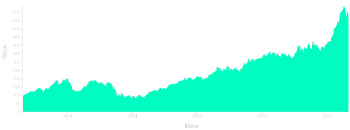
\includegraphics[width=0.95\textwidth]{figures/chap2/areachart.png}
  \captionof{figure}[Screenshot Area Chart Wizard]{Screenshot Area Chart Wizard
\label{fig_areachart}}
\end{center}

\textbf{Code areachart.html}

Omdat veel code weergeven moeilijk gaat in een document verwijs ik u naar de broncode indien ze niet leesbaar is.
\begin{lstlisting}
<!DOCTYPE html>
<html>

<head>
        <meta http-equiv="Content-Type" content="text/html; charset=ISO-8859-1">
        <title>Area Chart</title>

        <!--CSS for every chart wizard-->
        <link href="css/charts.css" rel="stylesheet" />

        <!--jQuery UI-->
        <link href="css/jquery-ui-1.10.4.custom.css" rel="stylesheet" />

        <!--Scrollbar-->
        <link href="css/jquery.mCustomScrollbar.css" rel="stylesheet" type="text/css" />

        <!--Main Menu-->
        <link href="css/main-menu.css" rel="stylesheet" type="text/css" />

        <!--Loading animation-->
        <link href="css/loading-balls.css" rel="stylesheet" type="text/css" />

        <!--Color picker-->
        <link rel="stylesheet" media="screen" type="text/css" href="css/colorpicker.css" />

        <!--Icons-->
        <link href="css/glyphicons.css" rel="stylesheet" />
</head>
\end{lstlisting}

In de head van de HTML pagina zetten we alle referenties naar de CSS paginas die we gebruiken voor deze pagina. De titel van de pagina is de titel die wordt weergegeven in je browser bovenaan in het tabblad.
\begin{lstlisting}

<body>
        <nav id="menu-wrap">
                <div id="menu-trigger">Menu</div>
                <ul id="menu">
                        <li id="disabled">&nbsp;</li>
                        <li><a href="home2.html">Home</a>
                        </li>
                        <li> <a href="#">Charts <b class="caret"></b></a>
                                <ul>
                                        <li><a href="areachart2.html">Area Chart</a>
                                        </li>
                                        <li><a href="barchart2.html">Bar Chart</a>
                                        </li>
                                        <li><a href="donutchart2.html">Donut Chart</a>
                                        </li>
                                        <li><a href="#">Bivariate Area Chart</a>
                                        </li>
                                        <li><a href="#">Grouped Bar Chart</a>
                                        </li>
                                        <li><a href="linechart2.html">Line Chart</a>
                                        </li>
                                        <li><a href="#">Multi-Line Chart</a>
                                        </li>
                                        <li><a href="piechart2.html">Pie Chart</a>
                                        </li>
                                        <li><a href="#">Scatterplot</a>
                                        </li>
                                </ul>
                        </li>
                        <li><a href="infographic.html">Infographics</a>
                        </li>
                        <li><a href="jezuscampraptorravepage.html">Help</a>
                        </li>
                        <li><a href="#about">About</a>
                        </li>
                        <li><a href="#contact">Contact</a>
                        </li>
        </nav>
        <div id="small-menu">
                <ul>
                        <li><a href="#" onClick="showDataDialog()">Data</a>
                        </li>
                        <li><a href="#" onClick="showAxesDialog()">Axes</a>
                        </li>
                        <li><a href="#" onClick="showAreaDialog()">Area</a>
                        </li>
                        <li><a href="#" onClick="showMovingAverageDialog()">Add</a>
                        </li>
                        <li><a href="#" onClick="showColorsDialog()">Color</a>
                        </li>
                        <li><a href="#" onClick="showTextDialog()">Text</a>
                        </li>
                        <li><a href="#" onClick="showExportDialog()">Export</a>
                        </li>
                </ul> 
        </div>                               
\end{lstlisting}

Het eerste deel van de body bevat de semantische opmaak van de twee menus. Het algemene navigatie menu en alle knoppen voor de wizard. In het algemene menu wordt nog een extra item toegevoegd in het begin en op het einde dat geen link bevat maar alleen dient als opmaak. De knoppen voor de wizard hebben allemaal een onClick event dat gekoppeld is aan een jQuery functie die de dialoog vensters zal openen.

\begin{lstlisting}                
        <div id="container">
                <div id="areachart-container" class="chart-container">
                        <h2 id="areachartTitleID" class="title">Area Chart</h2>
                        <div class="areachartdiv" id="areachartdiv"></div>
                        <!--A canvas to copy the svg to when we're exporting it-->
                        <canvas width="960" height="500" style="display:none"></canvas>
                </div>
        </div>
\end{lstlisting}

In deze container zit het div element waar de chartwizard-library een SVG element en de rest van de chart in zal tekenen. Er is ook een head element voor de titel van de chart die aangepast kan worden. En een canvas dat niet weergegeven wordt dat gebruikt wordt voor de SVG te exporteren naar een png figuur.

\begin{lstlisting}
        <!--Dialogs-->
        <div id="data-dialog" title="Data Settings" class="dialog">
                <div class="btn-group">
                        <div class="fileinput fileinput-new" data-provides="fileinput">
                                <div class="input-group">
                                        <input id="input-file" type="file" name="..." onChange="updateChart()">
                                        <a id="csv-upload" href="#" class="btnz" data-dismiss="fileinput" onClick="clearChart()">Remove</a> 
                                </div>
                                <button type="button" class="btnz btn-default" onClick="updateChart()" style="margin-top:10px; margin-bottom:10px">Generate Chart</button>
                        </div>
                </div>
        </div>
        <div id="axes-dialog" title="Axes Settings" class="dialog">
                <div class="row">
                        <div class="col-lg-6">
                                <p>X Axis Name</p>
                                <input id="xaxis-name" type="text" class="form-input" placeholder="X Axis" onChange="charts.chart.Areachart.Generate.UpdateXaxisName(this.value)" value="Date">
                        </div>
                        <div class="col-lg-6">
                                <p>Y Axis Name</p>
                                <input id="yaxis-name" type="text" class="form-input" placeholder="Y Axis" onChange="charts.chart.Areachart.Generate.UpdateYaxisName(this.value)" value="Value">
                        </div>
                </div>
        </div>
        <div id="area-dialog" title="Area Settings" class="dialog">
                <h3>Interpolation</h3>
                Sets the interpolation mode to the specified function. The following named interpolation modes are supported:
                <div class="btn-group">
                        <label class="btnz btn-primary">
                                <input type="radio" name="options" id="linear-option-btn" onChange="checkOptionsState()" data-toggle="button">Linear</label>
                        <label class="btnz btn-primary">
                                <input type="radio" name="options" id="step-option-btn" onChange="checkOptionsState()" data-toggle="button">Step</label>
                        <label class="btnz btn-primary">
                                <input type="radio" name="options" id="basis-option-btn" onChange="checkOptionsState()" data-toggle="button">Basis</label>
                        <label class="btnz btn-primary">
                                <input type="radio" name="options" id="bundle-option-btn" onChange="checkOptionsState()" data-toggle="button">Bundle</label>
                        <label class="btnz btn-primary">
                                <input type="radio" name="options" id="cardinal-option-btn" onChange="checkOptionsState()" data-toggle="button">Cardinal</label>
                        <label class="btnz btn-primary">
                                <input type="radio" name="options" id="monotone-option-btn" onChange="checkOptionsState()" data-toggle="button">Monotone</label>
                </div>
                <div id="area-options-description">
                        <h3>Description</h3>
                        No interpolation mode selected.</div>
        </div>
        <div id="moving-average-dialog" title="Add a Moving Average Line" class="dialog">
                <p>Show Moving Average Line</p>
                <input type="checkbox" onClick="charts.chart.Areachart.Generate.MovingAverage(this.checked)">
        </div>
        <div id="colors-dialog" title="Color Settings" class="dialog">
                <p>Area Color</p>
                <span style="height:64px; width:64px;">
  <div id="area-color-picker" class="color-picker">
    <div style="background-color: steelblue;"> </div>
  </div>
  </span>
                <p>Area Opacity</p>
                <div id="opacity-slider" style="width:200px;"></div>
        </div>
        <div id="text-dialog" title="Text Settings" class="dialog">
                <p>Chart Title</p>
                <input id="chart-title" type="text" value="Area Chart" class="form-input" onChange="UpdateChartTitle(this.value)">
                <p>Text & Axis Color</p>
                <span style="height:64px; width:64px;">
  <div id="text-color-picker" class="color-picker">
    <div style="background-color: #07FFC1;"> </div>
  </div>
  </span> 
        </div>
        <div id="export-dialog" title="Export" class="dialog">
                <button type="button" class="btnz" onClick="GenerateSVG()">Export SVG</button>
                <button type="button" class="btnz" onClick="GenerateHTML()">Export HTML</button>
                <button type="button" class="btnz" onClick="GenerateJPEG()">Download PNG</button>
        </div>
        </div>
        <div class="footer-wrapper">
                <div id="footer">Developed by Dries Crauwels</div>
        </div>
\end{lstlisting}

Alle dialoogvensters voor de chart te bewerken zijn jQuery UI elementen. En worden dus ook gestijld door je eigen jQuery CSS. Deze dialoog vensters komen altijd vooraan te staan en je kan ze slepen waar je wilt. 

\begin{lstlisting}
        <!-- jQuery -->
        <script src="https://ajax.googleapis.com/ajax/libs/jquery/1.11.0/jquery.min.js"></script>

        <!--D3 Library-->
        <script src="http://d3js.org/d3.v3.min.js"></script>

        <!-- Some library for tooltips-->
        <script src="http://labratrevenge.com/d3-tip/javascripts/d3.tip.v0.6.3.js"></script>

        <!---Custom chart wizard library-->
        <script src="js/chartwizard-library.js"></script>

        <!--Spinner-->
        <script src="js/spin.js"></script>

        <!--JQuery UI -->
        <script src="js/jquery-ui-1.10.4.js"></script>

        <!--Color picker-->
        <script type="text/javascript" src="js/colorpicker.js"></script>
        
        
\end{lstlisting}

Een HTML pagina wordt van boven naar beneden ingelezen. De volgorde waarin we de externe javascript libraries inladen is dus van belang. Als we onze eigen library eerst in laden voor die van D3 zelf zal deze niet werken omdat ze de D3 library nodig heeft.

\begin{lstlisting}        
        
        <script>
                     
                     
                 /////////////////////////////////////////////////////////////////////////////////////////////////////////////////////////////
                 //////////////////////////////////////////////////INITIALISATIONS////////////////////////////////////////////////////////////
                 /////////////////////////////////////////////////////////////////////////////////////////////////////////////////////////////	


                $(document).ready(function () {


                        //Get the CSV data, then generate the chart as callback
                        charts.readCSV("areachartdata2.csv", function (outputdata) {

                                data = outputdata;



                                charts.chart("AreaChart");
                                charts.chart.Areachart("#areachartdiv");
                                charts.chart.Areachart.Generate(data);

                        });
                });

\end{lstlisting}

De document.ready functie is een jQuery functie die wordt uitgevoerd wanneer het HTML document volledig is binnengehaald. Dit wil zeggen als de gebruiker dus niet meer moet wachten op het laden. Hierin kunnen we dan andere functies zetten die moeten worden uitgevoerd als dit is gebeurd. We zetten hierin de functie van de eigen chartwizard-library om de chart te tekenen met zijn initiele data.

In javascript kunnen we eender welke functie uitvoeren na dat een andere functie klaar is. Een callback heet dit. Dit hebben we hier nodig omdat als we niet eerst wachten tot de CSV file is ingelezen en de data in een array is gestopt, dan tekenen we de chart al zonder data en krijgen we niets te zien. De CSV inlezen is een asynchrone functie van D3 en het tekenen van de chart moet synchroon gebeuren.

charts.chart("Areachart") zegt ons dat we een areachart willen tekenen. Dus dat we in deze case van de switch-case zitten. Daarna zeggen we in welke div we de SVG willen tekenen.
De output van de readCSV() functie is een array van objecten en deze geven we mee aan de laatste functie die de chart effectief zal tekenen.
\begin{lstlisting}
                 /////////////////////////////////////////////////////////////////////////////////////////////////////////////////////////////
                 //////////////////////////////////////////////////JQUERY UI//////////////////////////////////////////////////////////////////
                 /////////////////////////////////////////////////////////////////////////////////////////////////////////////////////////////


                 //Give the buttons the jQuery style

                $(".btnz").button();

                 //Color picker widget
                $('#text-color-picker').ColorPicker({
                        //Default value
                        color: '#000',
                        onShow: function (colpkr) {
                                $(colpkr).fadeIn(500);
                                return false;
                        },
                        onHide: function (colpkr) {
                                $(colpkr).fadeOut(500);
                                return false;
                        },
                        onChange: function (hsb, hex, rgb) {
                                //Change color of country
                                changeChartTextColor((hex));
                                //Change background of color picker
                                $('#text-color-picker div').css('backgroundColor', '#' + hex);
                                //Set a global variable that we need when we turn off or on the grid
                                chartTextColor = hex;
                        }
                });
                $('#area-color-picker').ColorPicker({
                        //Default value
                        color: '#000',
                        onShow: function (colpkr) {
                                $(colpkr).fadeIn(500);
                                return false;
                        },
                        onHide: function (colpkr) {
                                $(colpkr).fadeOut(500);
                                return false;
                        },
                        onChange: function (hsb, hex, rgb) {
                                //Change color of country
                                charts.chart.Areachart.Generate.UpdateAreaColor(hex);
                                //Change background of color picker
                                $('#area-color-picker div').css('backgroundColor', '#' + hex);

                        }
                });


                $('#data-dialog').dialog({
                        autoOpen: false,
                        title: 'Import Your Data',
                        modal: false,
                        resizable: false,
                        height: 220,
                        width: 450
                });

                $('#axes-dialog').dialog({
                        autoOpen: false,
                        title: 'Axes Settings',
                        modal: false,
                        resizable: false,
                        height: 240,
                        width: 550
                });

                $('#area-dialog').dialog({
                        autoOpen: false,
                        title: 'Area Settings',
                        modal: false,
                        resizable: false,
                        height: 300,
                        width: 740
                });

                $('#moving-average-dialog').dialog({
                        autoOpen: false,
                        title: 'Add a Moving Average Line',
                        modal: false,
                        resizable: false,
                        height: 240,
                        width: 450
                });

                $('#colors-dialog').dialog({
                        autoOpen: false,
                        title: 'Color Settings',
                        modal: false,
                        resizable: false,
                        height: 220,
                        width: 400
                });

                $('#text-dialog').dialog({
                        autoOpen: false,
                        title: 'Text Settings',
                        modal: false,
                        resizable: false,
                        height: 220,
                        width: 450
                });

                $('#export-dialog').dialog({
                        autoOpen: false,
                        title: 'Export Your Chart',
                        modal: false,
                        resizable: false,
                        height: 220,
                        width: 450
                });

                $(function () {
                        $("#opacity-slider").slider({
                                value: 100,
                                min: 0,
                                max: 100,
                                step: 1,
                                slide: function (event, ui) {
                                        charts.chart.Areachart.Generate.UpdateOpacity(ui.value);

                                }
                        })
                        $("#opacity-slider").val($("#opacity-slider").slider("value"));
                });

                 //Dialogs
                function showDataDialog() {
                        $("#data-dialog").dialog("open");
                }

                function showAxesDialog() {
                        $("#axes-dialog").dialog("open");
                }

                function showAreaDialog() {
                        $("#area-dialog").dialog("open");
                }

                function showMovingAverageDialog() {
                        $("#moving-average-dialog").dialog("open");
                }

                function showColorsDialog() {
                        $("#colors-dialog").dialog("open");

                }

                function showTextDialog() {
                        $("#text-dialog").dialog("open");
                }

                function showExportDialog() {
                        $("#export-dialog").dialog("open");
                }

                function checkOptionsState() {
                        if ($("#linear-option-btn").prop("checked") == true) {
                                charts.chart.Areachart.Generate.UpdateArea("linear");
                                document.getElementById("area-options-description").innerHTML = ("<h3>Description</h3> Piecewise linear segments, as in a polyline.");
                        }
                        if ($("#step-option-btn").prop("checked") == true) {
                                charts.chart.Areachart.Generate.UpdateArea("step");
                                document.getElementById("area-options-description").innerHTML = ("<h3>Description</h3> Alternate between horizontal and vertical segments, as in a step function.");
                        }
                        if ($("#basis-option-btn").prop("checked") == true) {
                                charts.chart.Areachart.Generate.UpdateArea("basis");
                                document.getElementById("area-options-description").innerHTML = ("<h3>Description</h3> A <a style='color:#99CCFF' target='_blank' href='http://en.wikipedia.org/wiki/B-spline'>B-spline</a>, with control point duplication on the ends.");
                        }
                        if ($("#bundle-option-btn").prop("checked") == true) {
                                charts.chart.Areachart.Generate.UpdateArea("bundle");
                                document.getElementById("area-options-description").innerHTML = ("<h3>Description</h3> Equivalent to basis, except the tension parameter is used to straighten the spline.");
                        }
                        if ($("#cardinal-option-btn").prop("checked") == true) {
                                charts.chart.Areachart.Generate.UpdateArea("cardinal");
                                document.getElementById("area-options-description").innerHTML = ("<h3>Description</h3> A <a style='color:#99CCFF'  target='_blank' href='http://en.wikipedia.org/wiki/Cubic_Hermite_spline#Cardinal_spline'> Cardinal spline</a>, with control point duplication on the ends.");

                        }
                        if ($("#monotone-option-btn").prop("checked") == true) {
                                charts.chart.Areachart.Generate.UpdateArea("monotone");
                                document.getElementById("area-options-description").innerHTML = ("<h3>Description</h3> <a style='color:#99CCFF' target='_blank' href='http://en.wikipedia.org/wiki/Monotone_cubic_interpolation'> Cubic interpolation</a> that preserves monotonicity in y.");
                        }
                        if ($("#normal-option-btn").prop("checked") == true) {
                                charts.chart.Areachart.Generate.UpdateArea("none");
                                document.getElementById("area-options-description").innerHTML = ("<h3>Description</h3>No interpolation mode selected.");
                        }

                }
\end{lstlisting}

Elk jQuery interface element moet geinitialiseerd worden. Dit gebeurt allemaal in bovenstaande code. Verder is er ook nog de instellingen voor een color-picker-widget van een externe library.

Indien nodig worden ook nog de functies uitgevoerd bij het aanpassen van de waardes van deze elementen. Zo wordt de kleur veranderd van de chart als we die in de color-picker veranderen. De aangeduidde interpolatie functie wordt uitgevoerd als de radio-button gecheckt staat en we kunnen ook de opacity van de chart aanpassen.

\begin{lstlisting}
                 /////////////////////////////////////////////////////////////////////////////////////////////////////////////////////////////
                 //////////////////////////////////////////////////JAVASCRIPT/////////////////////////////////////////////////////////////////
                 /////////////////////////////////////////////////////////////////////////////////////////////////////////////////////////////
\end{lstlisting}

Onder de JavaScript comment komt alle overige code die nodig is voor de chart te bewerken. Er kan jQuery of D3 code gebruikt worden maar er wordt niets gestijld of ge\"{i}nitialiseerd.

\begin{lstlisting}
                var chartTextColor = "";

                function changeChartTextColor(inputcolor) {
                        chartTextColor = "#" + inputcolor;

                        var xAxisText = d3.selectAll(".areachart .xAxis text");
                        var xAxisLines = d3.selectAll(".areachart .xAxis line");
                        var xAxis = d3.selectAll(".areachart .xAxis path");

                        xAxisText.style("fill", chartTextColor);
                        xAxisLines.style("stroke", chartTextColor);
                        xAxis.style("stroke", chartTextColor);

                        var yAxisText = d3.selectAll(".areachart .yAxis text");
                        var yAxisLines = d3.selectAll(".areachart .yAxis line");
                        var yAxis = d3.selectAll(".areachart .yAxis path");

                        yAxisText.style("fill", chartTextColor);
                        yAxisLines.style("stroke", chartTextColor);
                        yAxis.style("stroke", chartTextColor);

                        $("#areachartTitleID").css("color", chartTextColor);

                }
\end{lstlisting}

Bovenstaande functie doet de kleur van de tekst veranderen op de assen, de assen zelf en de titel van de chart. We selecteren de text, line en path elementen en veranderen dan hun attribuutwaarden. Belangrijk om te weten is dat we voor de tekst het attribuut "fill" in de style moeten aanpassen en niet "color". Voor de lijnen is het "stroke". Ten slotte voor de titel dat buiten het SVG element staat, kunnen we jQuery code gebruiken om deze te selecteren en zijn "color" style aan te passen.

\begin{lstlisting}
                function GenerateSVG() {
                        var html = d3.select(".areachart")
                                .attr("title", "areachartdiv")
                                .attr("version", 1.1)
                                .attr("xmlns", "http://www.w3.org/2000/svg")
                                .node().parentNode.innerHTML;

                        var newwindow = window.open('', 'name', 'height=400,width=1000');




                        var newwindowroot = d3.select(newwindow.document.body).append("div")
                                .attr("id", "SVG")
                                .append("img")
                                .attr("src", "data:image/svg+xml;base64," + btoa(html));
                }

                function GenerateHTML() {
                        var html = d3.select("#areachartdiv")
                                .attr("title", "areachartdiv")
                                .attr("version", 1.1)
                                .attr("xmlns", "http://www.w3.org/2000/svg")
                                .node().parentNode.innerHTML;

                        var newwindow = window.open('', 'name', 'height=400,width=1000');

                        newwindow.document.write(html);
                        newwindow.document.write("<textarea>");
                        newwindow.document.write(html);
                        newwindow.document.write("</textarea>");

                        return html;

                }

                function GenerateJPEG() {




                        var html = d3.select(".areachart")
                                .attr("title", "areachartdiv")
                                .attr("version", 1.1)
                                .attr("xmlns", "http://www.w3.org/2000/svg")
                                .node().parentNode.innerHTML;

                        var imgsrc = 'data:image/svg+xml;base64,' + btoa(html);
                        var img = '<img src="' + imgsrc + '">';
                        //d3.select("#svgdataurl").html(img);

                        var canvas = document.querySelector("canvas");
                        var context = canvas.getContext("2d");

                        //Clear the canvas incase we drew something on the canvas already from exporting before
                        // Store the current transformation matrix
                        context.save();

                        // Use the identity matrix while clearing the canvas
                        context.setTransform(1, 0, 0, 1, 0, 0);
                        context.clearRect(0, 0, canvas.width, canvas.height);

                        // Restore the transform
                        context.restore();

                        var image = new Image;
                        image.src = imgsrc;
                        image.onload = function () {

                                context.drawImage(image, 0, 0);

                                var canvasdata = canvas.toDataURL("image/jpg");

                                var pngimg = '<img src="' + canvasdata + '">';
                                //d3.select("#pngdataurl").html(pngimg);

                                var a = document.createElement("a");
                                a.download = "sample.jpg";
                                a.href = canvasdata;
                                a.click();
                        };
                }
\end{lstlisting}

Het exporteren zal altijd een nieuw venster openen dat laat zien wat je krijgt. Niet alles kan ge\"{e}xporteerd worden. De mouse-over events worden niet mee doorgegeven als we de HTML exporteren omdat deze in de chartwizard-library zitten. Net zoals de CSS die in een extern bestand kan zitten. Je moet dus de CSS van de charts inline in de code zetten.
 
De functies om de chart te exporteren naar een SVG, HTML of PNG bestand zijn niet zo eenvoudig.
Om te exporteren naar een SVG bestand komt het erop neer om het volledige SVG element te selecteren en dit om te zetten naar base 64 data om het in de "src" van een \textless img\textgreater element te stoppen. De gebruiker kan dan op de rechtermuisknop klikken om de SVG op te slaan.

De HTML exporteren is niet al te ingewikkeld. We selecteren de volledige innerHTML van de \textless div\textgreater waar de SVG in zit en laten deze zien in een nieuw venster en in een textarea zodat we deze makkelijk kunnen kopieren.  

Het exporteren naar een PNG is het meest ingewikkelde. De innerHTML van de \textless div\textgreater waar de chart in zit wordt geselecteerd en deze wordt gekopieerd naar een HTML canvas element. Indien we dit meerdere keren willen doen moet het canvas uiteraard altijd leeggemaakt worden voor we iets neiuws tekenen. Een post op Stackoverflow[1] legt uit hoe dit op verschillende manieren kan. Daarna kunnen we een functie aanroepen die eigen is aan het canvas element om alles wat hierin getekend is te rasterizen naar een PNG bestand.

\begin{itemize}
 \item $[1]$: \url{http://stackoverflow.com/questions/2142535/how-to-clear-the-canvas-for-redrawing}
\end{itemize}
\begin{lstlisting}

                function ReadCSV() {
                        var stringpath = document.getElementById("input-file").value;
                        return stringpath.slice(12);
                }
\end{lstlisting}

Het inlezen van de CSV geeft de naam van het bestand dat we hebben gekozen in het Data dialoogvenster terug. Als we de waarde van het element met het ID input-file opvragen is dit een string met het pad van het bestand. Hiervan laten we dan de eerste 12 karakters weg om alleen de bestandsnaam te krijgen.

Merk op dat deze bestanden in de map zitten naast de andere .HTML bestanden en we gewoon andere selecteren. Er is geen upload functie die bestanden op de server zet en deze inleest.

\begin{lstlisting}
                function UpdateChartTitle(inputtext) {
                        document.getElementById("areachartTitleID").innerHTML = inputtext;
                }
\end{lstlisting}

Functie om de titel van de chart te veranderen naar de text input.

\begin{lstlisting}
                function updateChart() {
                        clearChart();
\end{lstlisting}

De chart updaten is simpelweg alle elementen in het SVG element verwijderen. Niet het SVG element zelf. En dan de chart opnieuw genereren met de nieuwe data.

\begin{lstlisting}

                        charts.getCSV(ReadCSV(), function (outputdata) {

                                data = outputdata;

                                charts.chart.Areachart.Generate(data);

                        });

                }

                function clearChart() {

                        d3.selectAll(".area").remove();
                        d3.selectAll(".average").remove();
                        d3.selectAll(".xAxis").remove();
                        d3.selectAll(".yAxis").remove();
                }
        </script>
</body>

</html>
\end{lstlisting}

\textbf{Code chartwizard-library.js voor de area chart}
\begin{lstlisting}[gobble=16]

			case "AreaChart":

                        charts.chart.Areachart = function (divclass) {
							
                                var areachart1 = d3.select(divclass)
                                        .append("svg")
                                        .attr("width", svgWidth + margin.left + margin.right)
                                        .attr("height", svgHeight + margin.top + margin.bottom)
                                        .attr("class", "areachart")
                                        .append("g")
                                        .attr("transform", "translate(" + (70) + "," + (20) + ")");

\end{lstlisting}

De eerste functie in de chartwizard-library van elke stuk code voor een chart te genereren bestaat uit een SVG element te tekenen in een \textless div\textgreater. Je geeft de classname mee als parameter en je krijgt een SVG element terug met daarin een \textless g\textgreater element. Een \textless g\textgreater element is een tag om andere elementen te groeperen. Dit maakt het makkelijker om groepen en subgroepen te maken om je chart elementen te ordenen.

\begin{lstlisting}[gobble=24]

                                charts.chart.Areachart.Generate = function (inputdata) {
                                        var data = inputdata;

                                        var parseDate = d3.time.format("%d-%b-%y").parse;

                                        var x = d3.time.scale()
                                                .range([0, svgWidth]);

                                        var y = d3.scale.linear()
                                                .range([svgHeight, 0]);
\end{lstlisting}

De inputdata die wordt meegegeven aan de Generate() functie is een array van objecten. Deze array komt van het inlezen van het CSV bestand. De parseDate variabele is een functie(javascript variabelen kunnen ook functies zijn) van D3 om de datum te parsen. De x en y variabelen zijn arrays van minimum en maximum waarden die worden berekent met de scale functies binnen D3. Omdat de chart een maximum vaste breedte en hoogte heeft moeten we de data altijd herschalen naar deze waarden. Het kan zijn dat er te veel data is en alles te dicht opeen staat en dat de chart gewoon te klein is. Als dit het geval is moet de gebruiker dit zelf inzien en minder data meegeven in de CSV. Een goede uitleg over hoe het schalen werkt binnen D3 vind je hieronder.

\url{http://chimera.labs.oreilly.com/books/1230000000345/ch07.html}

\begin{lstlisting}[gobble=24]
                                        var xAxis = d3.svg.axis()
                                                .scale(x)
                                                .orient("bottom");

                                        var yAxis = d3.svg.axis()
                                                .scale(y)
                                                .orient("left");
\end{lstlisting}

De xAxis en yAxis variabelen stellen de assen voor. Hiervoor worden de x en y waarden gebruikt die hiervoor zijn berekend om de minimum en maximum in te stellen.

\begin{lstlisting}[gobble=24]
                                        var area = d3.svg.area()
                                                .x(function (d) {
										//Add +1 to move it one pixel to the right of the Y axis
                                                        return x(d.date)+1;
                                                })
                                                .y0(svgHeight)
                                                .y1(function (d) {
                                                        return y(d.close);
                                                });



                                        data.forEach(function (d) {
                                                d.date = parseDate(d.date);
                                                d.close = +d.close;
                                        });


                                        x.domain(d3.extent(data, function (d) {
                                                return d.date;
                                        }));
                                        y.domain([0, d3.max(data, function (d) {
                                                return d.close;
                                        })]);
\end{lstlisting}

Het berekenen van de waarden nodig om het path element te tekenen gebeurt hierboven. d.close en d.date verwijzen naar de data. close en date zijn de namen van de variabelen in de CSV. Dus als we die veranderen zal de code niet werken. Het is dus belangrijk dat de gebruiker weet dat hij zijn twee waarden de namen date en close moet geven in het CSV bestand. De chart is nog niet getekend.

\begin{lstlisting}[gobble=24]

                                        //remove previous chart if there was one
                                        areachart1.selectAll("path").remove();

                                        areachart1.append("path")
                                                .datum(data)
                                                .attr("class", "area")
                                                .attr("d", area)
                                                .style({
                                                        "fill": "steelblue"
                                                });
\end{lstlisting}

De data is nu in de juiste vorm om het gebied te tekenen. We geven ze een class name en tekenen het path element met een "fill" style voor de kleur.

\begin{lstlisting}[gobble=24]

                                        areachart1.select(".xAxis").remove();
                                        areachart1.select(".yAxis").remove();


                                        areachart1.append("g")
                                                .attr("class", "xAxis")
                                                .attr("transform", "translate(0," + svgHeight + ")")
                                                .call(xAxis)
                                                .append("text")
                                                .attr("class", "xAxisText")
                                                .attr("y", 50) 
                                                //Hoever van de as verwijdert
                                                //ten opzichte van de y as
                                        .attr("x", svgWidth / 2)
                                                .text("Date")
                                                .style({
                                                        "font-family": "sans-serif",
                                                        "font-size": 18,
														"color":"#CCC"
                                                });;

                                        areachart1.append("g")
                                                .attr("class", "yAxis")
                                                .call(yAxis)
                                                .append("text")
                                                .attr("class", "yAxisText")
                                                .attr("transform", "rotate(-90)")
                                                .attr("y", -50)
                                                .attr("x", -svgHeight / 2)
                                                .text("Value")
                                                .style({
                                                        "font-family": "sans-serif",
                                                        "font-size": 18,
														"color":"#CCC"
                                                });

                                        //inline CSS styling

                                        areachart1.selectAll(".domain")
                                                .style({
                                                        "fill": "none",
                                                        "stroke": "#CCC",
                                                        "shape-rendering": "crispEdges"
                                                });

                                        areachart1.selectAll("line")
                                                .style({
                                                        "fill": "none",
                                                        "stroke": "#CCC",
                                                        "shape-rendering": "crispEdges"
                                                });

                                        //Give all X values a class and style them
                                        areachart1.selectAll(".xAxis g text").attr("class", "xAxisValues")
                                                .style({
                                                        "font-family": "sans-serif",
                                                        "font-size": 12,
														"fill":"#CCC"
                                                });

                                        //Give all Y values a class and style them
                                        areachart1.selectAll(".yAxis g text").attr("class", "yAxisValues")
                                                .style({
                                                        "font-family": "sans-serif",
                                                        "font-size": 12,
														"fill":"#CCC"
                                                });
												
										//Color the axis names too
									areachart1.select(".xAxisText").style({"fill":"#ccc"});
									areachart1.select(".yAxisText").style({"fill":"#ccc"});

\end{lstlisting}

Het toevoegen van de assen is analoog met het gebied. Let op dat de assen wel in het \textless g\textgreater element zitten in de SVG en elke as nog is in een aparte \textless g\textgreater. Je kan nooit teveel \textless g\textgreater elementen tekenen. Net zoals er nooit te veel \textless div\textgreater elementen kunnen zijn. Zoals ervoor al is vermeld, wordt de styling inline gebeurt zodanig dat die wordt behouden bij het exporteren. De SVG moet \'e\'en geheel vormen en mag niets extern nodig hebben.

\begin{lstlisting}[gobble=24]


                                        //Calculate moving average
                                        // Setup the moving average calculation.
                                        // Currently is a hacky way of doing it by manually storing and using the previous 3 values for averaging.
                                        // Looking for another way to address previous values so we can make the averaging window much larger (like 15 previous values).
                                        var prevPrevVal = 0;
                                        var prevVal = 0;
                                        var curVal = 0
                                        var movingAverageLine = d3.svg.line()
                                                .x(function (d, i) {
                                                        return x(d.date);
                                                })
                                                .y(function (d, i) {
                                                        if (i == 0) {
                                                                prevPrevVal = y(d.close);
                                                                prevVal = y(d.close);
                                                                curVal = y(d.close);
                                                        } else if (i == 1) {
                                                                prevPrevVal = prevVal;
                                                                prevVal = curVal;
                                                                curVal = (prevVal + y(d.close)) / 2.0;
                                                        } else {
                                                                prevPrevVal = prevVal;
                                                                prevVal = curVal;
                                                                curVal = (prevPrevVal + prevVal + y(d.close)) / 3.0;
                                                        }
                                                        return curVal;

                                                })
                                                .interpolate("basis");

                                        //Draw moving average but don't show it yet
                                        areachart1.append("path")
                                                .attr("class", "average")
                                                .attr("d", movingAverageLine(data))
                                                .style({
                                                        "stroke": "darkviolet",
                                                        "stroke-width": 1,
                                                        "fill": "none",
                                                        "opacity": 0
                                                });
                                                
\end{lstlisting}

Als extra functionaliteit wordt hierboven een moving average lijn berekend en getekend. De lijn is echter wel nog doorzichtig. Dit wordt pas veranderd indien de gebruiker de checkbox aanzet voor het weergeven van de moving average. Herinner dat SVG elementen geen "z-index" hebben en dus worden gestapeld in volgorde van het tekenen. Het laatst toegevoegde element wordt dus bovenop de rest geplaatst. Het is dus belangrijk dat de moving average pas wordt getekend na het tekenen van het gebied om ze er bovenop te plaatsen.

\begin{lstlisting}[gobble=28]                                             
                                                
                                        charts.chart.Areachart.Generate.UpdateArea = function (inputsmoothingtype) {
											
                                                if (inputsmoothingtype == "linear") {

                                                        area = d3.svg.area()
                                                                .interpolate("linear")

                                                        .x(function (d) {
                                                                return x(d.date)+1;
                                                        })
                                                                .y0(svgHeight)
                                                                .y1(function (d) {
                                                                        return y(d.close);
                                                                });

                                                        areachart1.selectAll(".area").remove();

                                                        areachart1.append("path")
                                                                .datum(data)
                                                                .attr("class", "area")

                                                        .attr("d", area)
                                                                .style({
                                                                        "fill": "steelblue"
                                                                });
                                                }

                                                if (inputsmoothingtype == "step") {

                                                        area = d3.svg.area()
                                                                .interpolate("step")

                                                        .x(function (d) {
                                                                return x(d.date)+1;
                                                        })
                                                                .y0(svgHeight)
                                                                .y1(function (d) {
                                                                        return y(d.close);
                                                                });

                                                        areachart1.selectAll(".area").remove();

                                                        areachart1.append("path")
                                                                .datum(data)
                                                                .attr("class", "area")
                                                                .attr("d", area)
                                                                .style({
                                                                        "fill": "steelblue"
                                                                });
                                                }

                                                if (inputsmoothingtype == "basis") {

                                                        area = d3.svg.area()
                                                                .interpolate("basis")
                                                                .x(function (d) {
                                                                        return x(d.date)+1;
                                                                })
                                                                .y0(svgHeight)
                                                                .y1(function (d) {
                                                                        return y(d.close);
                                                                });

                                                        areachart1.selectAll(".area").remove();

                                                        areachart1.append("path")
                                                                .datum(data)
                                                                .attr("class", "area")
                                                                .attr("d", area)
                                                                .style({
                                                                        "fill": "steelblue"
                                                                });
                                                }

                                                if (inputsmoothingtype == "bundle") {

                                                        area = d3.svg.area()
                                                                .interpolate("bundle")
                                                                .x(function (d) {
                                                                        return x(d.date)+1;
                                                                })
                                                                .y0(svgHeight)
                                                                .y1(function (d) {
                                                                        return y(d.close);
                                                                });

                                                        areachart1.selectAll(".area").remove();

                                                        areachart1.append("path")
                                                                .datum(data)
                                                                .attr("class", "area")
                                                                .attr("d", area)
                                                                .style({
                                                                        "fill": "steelblue"
                                                                });
                                                }

                                                if (inputsmoothingtype == "cardinal") {

                                                        area = d3.svg.area()
                                                                .interpolate("cardinal")
                                                                .x(function (d) {
                                                                        return x(d.date)+1;
                                                                })
                                                                .y0(svgHeight)
                                                                .y1(function (d) {
                                                                        return y(d.close);
                                                                });

                                                        areachart1.selectAll(".area").remove();

                                                        areachart1.append("path")
                                                                .datum(data)
                                                                .attr("class", "area")
                                                                .attr("d", area)
                                                                .style({
                                                                        "fill": "steelblue"
                                                                });
                                                }

                                                if (inputsmoothingtype == "monotone") {

                                                        area = d3.svg.area()
                                                                .interpolate("monotone")
                                                                .x(function (d) {
                                                                        return x(d.date)+1;
                                                                })
                                                                .y0(svgHeight)
                                                                .y1(function (d) {
                                                                        return y(d.close);
                                                                });

                                                        areachart1.selectAll(".area").remove();

                                                        areachart1.append("path")
                                                                .datum(data)
                                                                .attr("class", "area")
                                                                .attr("d", area)
                                                                .style({
                                                                        "fill": "steelblue"
                                                                });
                                                }
                                                if (inputsmoothingtype == "none") {
													

													
                                                        area = d3.svg.area()
                                                                .interpolate("linear")
                                                                .x(function (d) {
                                                                        return x(d.date)+1;
                                                                })
                                                                .y0(svgHeight)
                                                                .y1(function (d) {
                                                                        return y(d.close);
                                                                });

                                                        areachart1.selectAll(".area").remove();

                                                        areachart1.append("path")
                                                                .datum(data)
                                                                .attr("class", "area")
                                                                .attr("d", area)
                                                                .style({
                                                                        "fill": "steelblue"
                                                                });

                                                }
                                        }
                                        
\end{lstlisting}

Dankzij D3 kunnen we het gebied manipuleren met ingebouwde wiskundige functies. We passen de area variabele aan naargelang welke interpolatie is gekozen door de gebruiker en tekenen de chart opnieuw. Denk eraan dat alleen de area variabele wordt aangepast en niet de data-array afkomstig van de CSV.

\begin{lstlisting}[gobble=28]                                        
                                         charts.chart.Areachart.Generate.MovingAverage = function (inputstate) {


                                                if (inputstate == true) {
													
														//Remove previous moving average line
                                                        areachart1.select(".average").remove();

                                                        areachart1.append("path")
                                                                .attr("class", "average")
                                                                .attr("d", movingAverageLine(data))
                                                                .style({
                                                                        "stroke": "darkviolet",
                                                                        "stroke-width": 1,
                                                                        "fill": "none",
                                                                        "opacity": 1
                                                                });


                                                        // Draw the moving average version of the data, as a line.

                                                } else
                                                        areachart1.select(".average")
                                                                .style({
                                                                        "opacity": 0
                                                                });
                                                //areachart1.select(".average").remove();
                                        }
                                        
\end{lstlisting}
                  
Om de moving average te plaatsen wordt alleen de opacity aangepast omdat de lijn al ervoor was getekend maar onzichtbaar was. De inputstate verwijst naar het feit of de checkbox aangeduid is of niet.                 
                                        
\begin{lstlisting}[gobble=24]                                       
                                        charts.chart.Areachart.Generate.UpdateYaxisName = function (inputtext) {
                                                yAxisText = inputtext;

                                                areachart1.select(".yAxisText")
                                                        .text(inputtext);
                                        }

                                        charts.chart.Areachart.Generate.UpdateXaxisName = function (inputtext) {
                                                xAxisText = inputtext;
                                                areachart1.select(".xAxisText")
                                                        .text(inputtext);
                                        }

                                        charts.chart.Areachart.Generate.UpdateAreaColor = function (inputcolor) {
                                                
                                                areachart1.select(".area")
                                                        .style({
                                                                "fill": inputcolor
                                                        });

                                        }

                                        charts.chart.Areachart.Generate.UpdateOpacity = function (inputvalue) {
                                                areachart1.select(".area")
                                                        .style({
                                                                "opacity": (inputvalue / 100)
                                                        });
                                        }

                                }

                        }

                        break;
                          
\end{lstlisting}

Ten slotte worden op het einde de update functies gezet om de chart aan te passen naar de wensen van de gebruiker. Steeds wordt het specifieke element geselecteerd met zijn class of ID en dan worden de attributen aangepast. Soms is dit niet mogelijk en moeten we de chart helemaal opnieuw tekenen. Het hangt ervan af wat je wilt veranderen.

\textbf{CSV bestand}
\begin{lstlisting}
date,close
1-May-12,13
30-Apr-12,98
27-Apr-12,0
26-Apr-12,70
25-Apr-12,0
24-Apr-12,28
23-Apr-12,170
20-Apr-12,98
19-Apr-12,44
18-Apr-12,34
17-Apr-12,70
16-Apr-12,12
13-Apr-12,23
12-Apr-12,77
11-Apr-12,20
10-Apr-12,44
9-Apr-12,23
5-Apr-12,68
4-Apr-12,31
3-Apr-12,32
2-Apr-12,63
30-Mar-12,55
29-Mar-12,86
28-Mar-12,62
27-Mar-12,48
26-Mar-12,98
23-Mar-12,05
22-Mar-12,34
21-Mar-12,50
\end{lstlisting}
\subsection{Bar Chart}

De bar chart wizard heeft net dezelfde functionaliteiten als de area chart wizard met nog een paar extra. Je kan de x waarden alfabetisch ordenen of volgens de y waarden van hoog naar laag. Er is ook een mouse-over functie om de huidige waarde van elke balk te laten weergeven. 

\begin{center}
  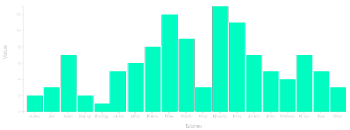
\includegraphics[width=0.95\textwidth]{figures/chap2/barchart.png}
  \captionof{figure}[Screenshot Bar Chart Wizard]{Screenshot Bar Chart Wizard
\label{fig_barchart}}
\end{center}

\textbf{CSV bestand}
\begin{lstlisting}
key,value
Joske,2
Jef,3
Jean,7
Danny,2
Freddy,1
Jules,5
Willy,6
Eddie,8
Nico,12
Mark,9
Amy,3
Klaudia,13
Inne,11
Jonah,7
Joke,5
Michael,4
Kirien ,7
Tess,5
Shari,3
\end{lstlisting}
\subsection{Donut Chart}

Een donut chart geeft de data volledig anders weer. De data wordt verdeeld over een volledige cirkel met een gat in het midden. Je kan de straal aanpassen om de cirkel groter of kleiner te maken, de kleur aanpassen en labels aan- of uitzetten.
\begin{center}
  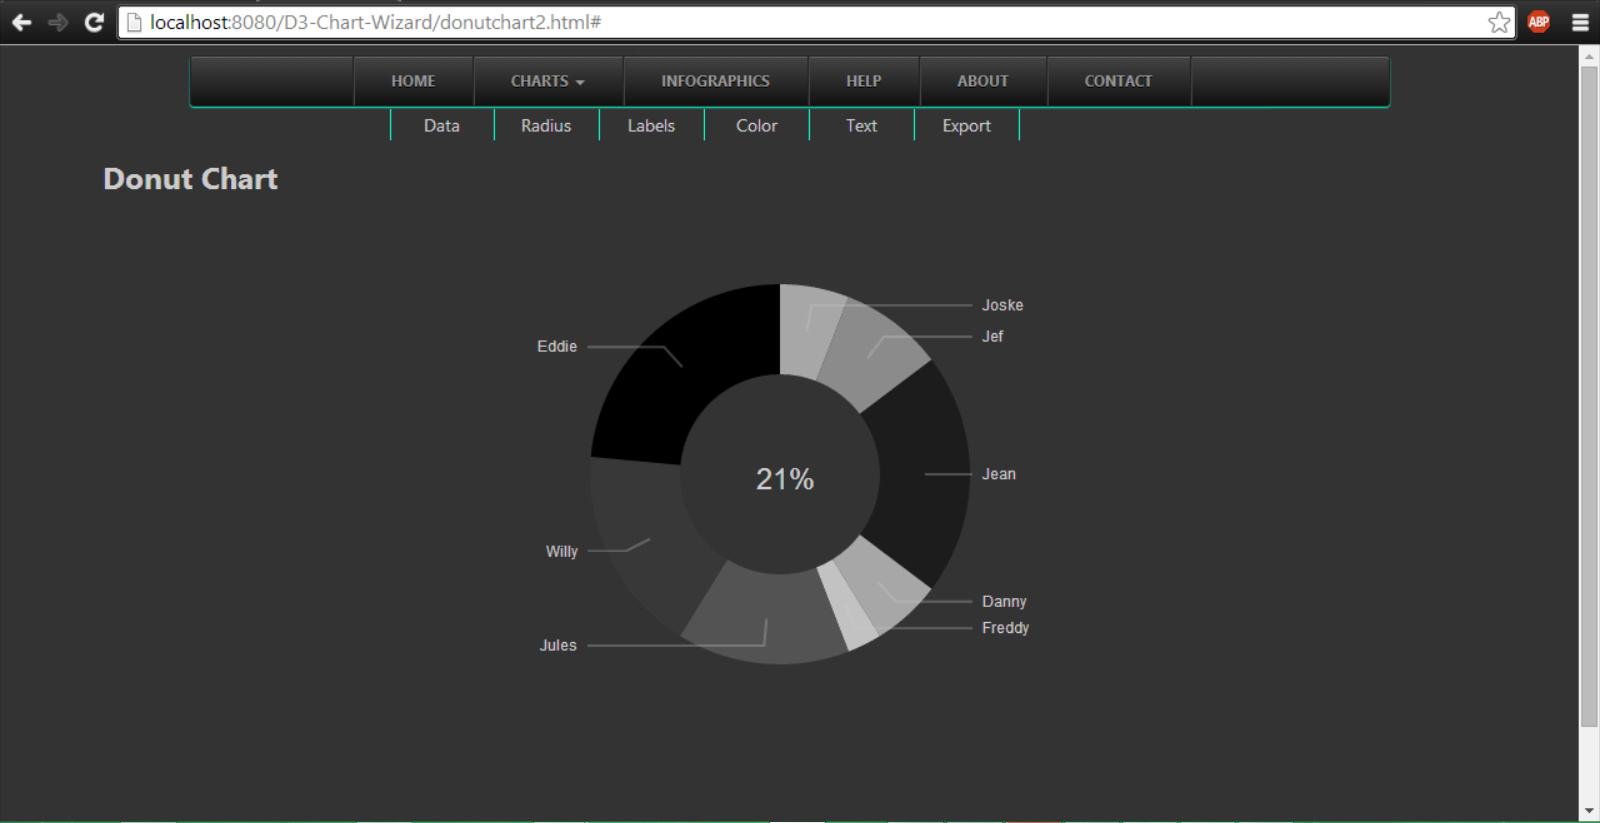
\includegraphics[width=0.95\textwidth]{figures/chap2/donutchart.png}
  \captionof{figure}[Screenshot Donut Chart Wizard]{Screenshot Donut Chart Wizard
\label{fig_donutchart}}
\end{center}

In dit voorbeeld wordt hetzelfde CSV bestand gebruikt als die van de bar chart.
\subsection{Line Chart}

De line chart wizard is identiek aan de area chart. Alleen is de lijn niet opgevuld. Om ervoor te zorgen dat deze wizard toch iets anders is, is er een mouse-over functie toegevoegd om de huidige waarde weer te geven. Dit is vooral handig als er veel waardes zijn. Jammer werkt deze mouse-over functie niet meer wanneer we de lijn veranderen met de interpolatie functies zoals in de area chart. Zoals eerder vermeld komt dit doordat de D3 functies alleen het path element veranderen en niet de data. De mouse-over functie volgt de data en geeft deze weer, niet het pad van de lijn.

\begin{center}
  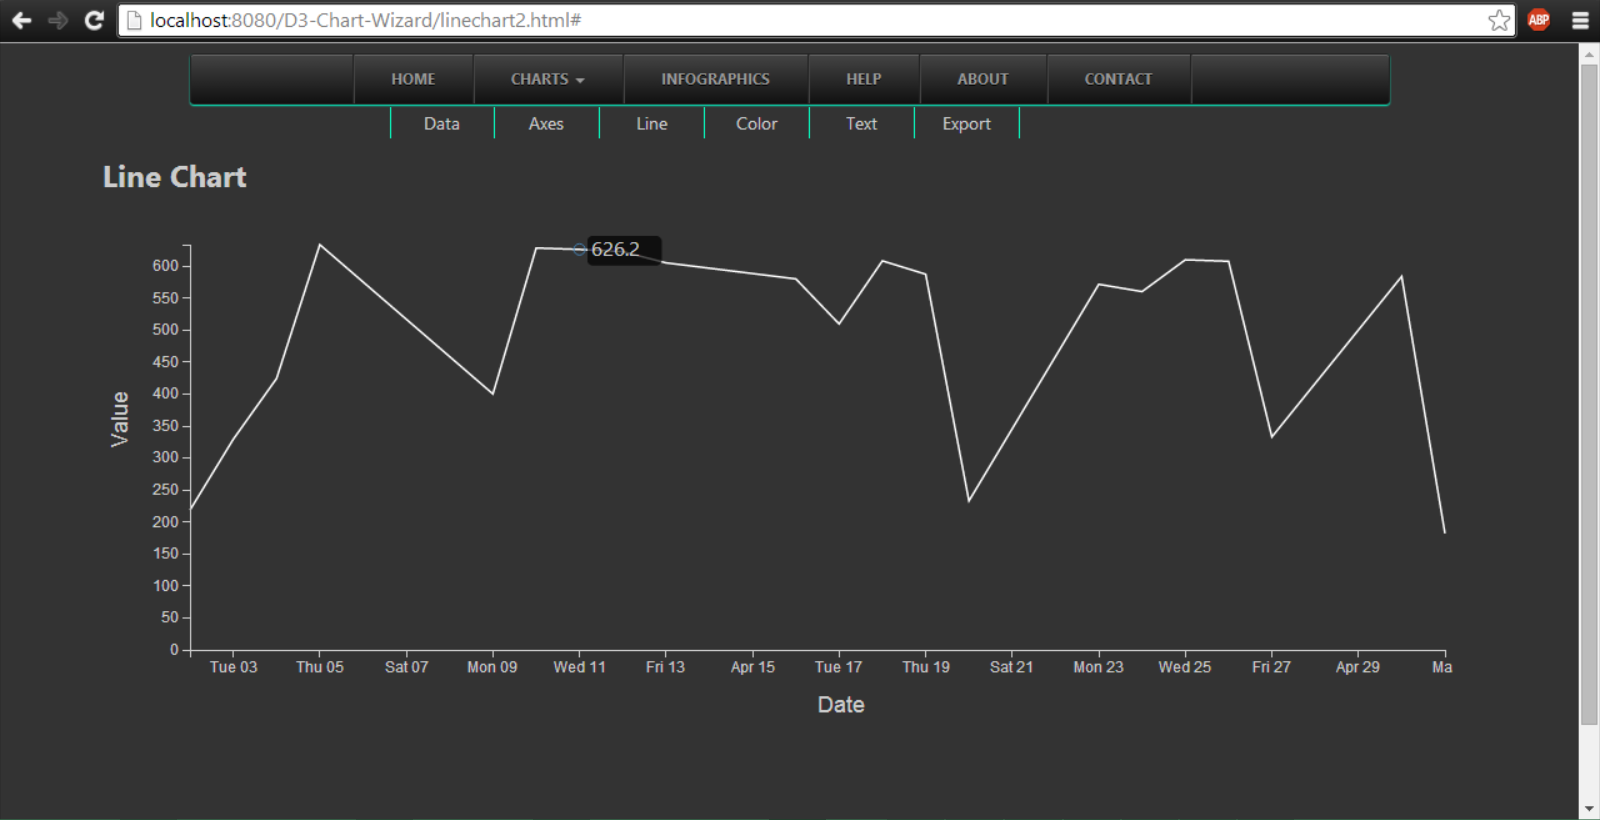
\includegraphics[width=0.95\textwidth]{figures/chap2/linechart.png}
  \captionof{figure}[Screenshot Line Chart Wizard]{Screenshot Line Chart Wizard
\label{fig_linechart}}
\end{center}

In dit voorbeeld wordt hetzelfde CSV bestand gebruikt als die van de area chart.
\section{Infographic Wizard}



Information Graphics of kortweg, infographics, zijn bedoeld om informatie te weergeven door middel van tekst en beeld. Dit kan simpelweg een paar pictrogrammen zijn of een hele uitleg rond de economische toestand van een land. Deze wizard is dan ook bedoeld om zoiets te kunnen nabootsen met de D3 library. Dit vraagt enorm veel code omdat de wizard de fantasie en ideeen van de gebruiker niet mag beperken. Met andere woorden alles moet mogelijk zijn. Deze applicatie is dan ook zeker niet volledig afgeraakt.

\begin{center}
  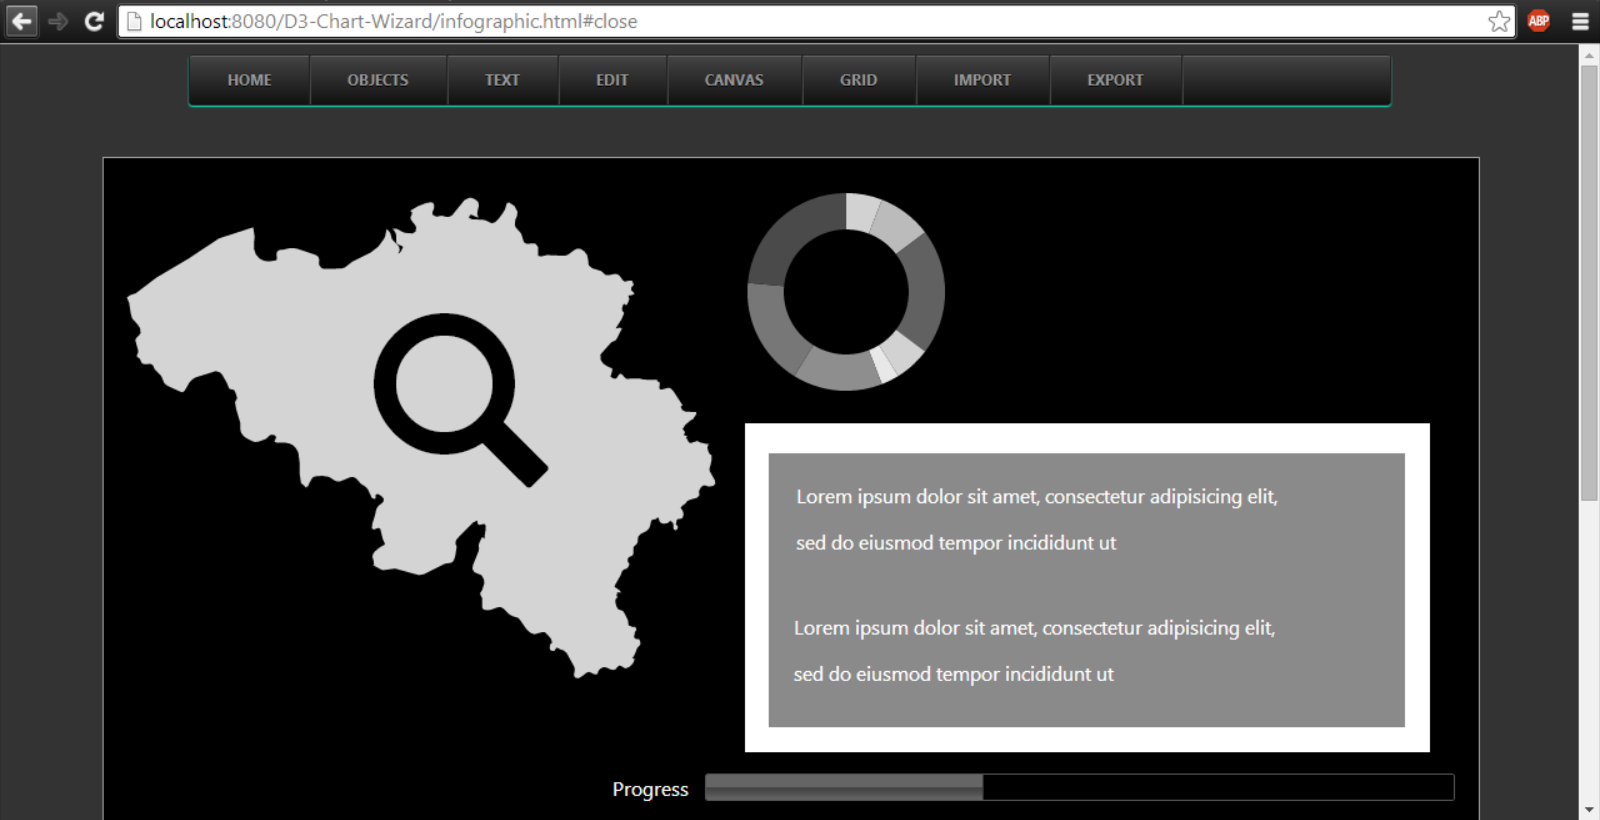
\includegraphics[width=0.95\textwidth]{figures/chap2/infographic.png}
  \captionof{figure}[Screenshot Infographic Wizard]{Screenshot Infographic Wizard
\label{fig_infographic}}
\end{center}

Bovenaan staat het menu met alle functionaliteiten. De algemene workflow, en ook de structuur van de code, is als volgt: je kiest wat voor object je wilt toevoegen en bewerkt deze in een mini wizard. Dan wordt deze gekopieerd en toegevoegd in het canvas met een unieke ID en kan je deze eender waar slepen. De unieke ID zorgt ervoor dat deze niet opnieuw geselecteerd wordt in de wizard als we nog eenzelfde object willen toevoegen. 

\begin{center}
  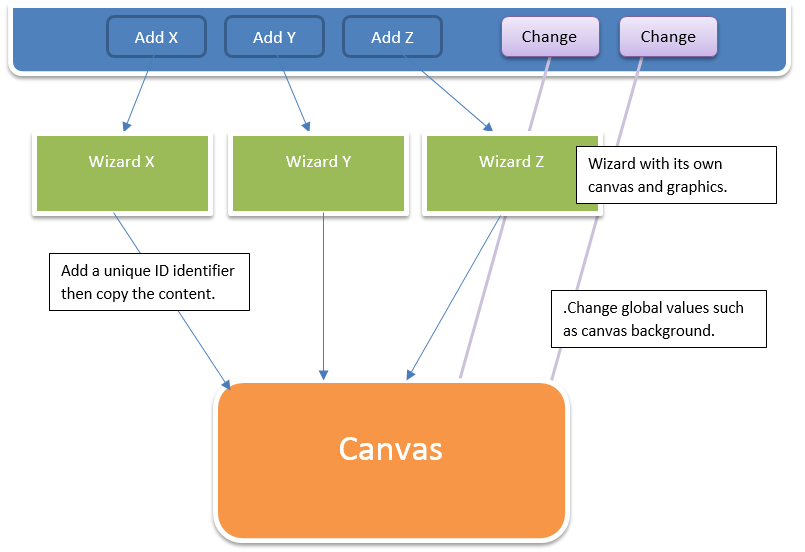
\includegraphics[width=0.95\textwidth]{figures/chap2/infographics-workflow.png}
\end{center}

Er is nog geen functionaliteit voorzien om deze objecten terug te selecteren en te bewerken. Je moet ze allemaal verwijderen en opnieuw beginnen als het niet naar wens is. Je kan ook een grid aanzetten dat altijd boven de objecten zal komen te staan om ze te ordenen. Je kan de resolutie van het canvas aanpassen en uiteraard ook tekst toevoegen.

De volgende objecten kunnen toegevoegd worden:

\begin{enumerate}
  \item Charts 
  		\begin{enumerate}
  			\item Donut Chart
  		\end{enumerate}
  \item Countries
  \item Icons
  \item Shapes
  \item Progress Bars
\end{enumerate}

De wizard voor de donut chart is min of meer dezelfde als die van ervoor. Alleen hier is ze iets compacter en is er geen export mogelijkheid omdat we ze in de infographic steken en die dan exporteren. De andere charts zijn nog niet toegevoegd.

Het uiteindelijke resultaat van de infographic is een mix van \textless div\textgreater en SVG elementen. Dit is geen ideale code omdat dit het heel lastig maakt om het te exporteren. We kunnen de SVG elementen exporteren maar niet met de \textless div\textgreater elementen erbij. Er is echter een element genaamd "foreign object"  binnen D3 dat gewone HTML elementen aanschouwt als SVG elementen.. Maar er was niet genoeg tijd om dit te testen en volledig uit te werken.

\url{https://gist.github.com/mbostock/1424037}

Totzover kun je kiezen uit 4 landen om toe te voegen. Dit komt omdat het geen gemakkelijke opdracht is om de data in de juiste vorm te krijgen en ze te dan te visualiseren. Indien we een land naar keuze willen toevoegen in onze code moeten we een aantal stappen ondernemen. 
Eerst downloaden we de wereld.

\url{http://www.naturalearthdata.com/downloads/10m-cultural-vectors/}

We kunnen dit shape bestand openen met QGIS.

\url{http://www.qgis.org/en/site/}

Open QGIS en sleep het shape bestand in de editor. Zorg ervoor dat de optie van bewerken aanstaat. Nu kan je eender welk land selecteren. Klik met de rechtermuisknop op het land en klik op save selection as geoJSON data. Nu hebben we de data, alleen staat deze nog niet in de vorm die D3 vraagt. Men moet deze nog comprimeren naar topoJSON data. Dit kan je doen op de volgende website:

\url{http://shancarter.github.io/distillery/}

Het is belangrijk te weten onder welk bestandsnaam je dit opslaat omdat er een variabele is die dezelfde naam heeft in de code. En deze zal gebruikt worden door D3 om de data in te lezen. Misschien is er snellere, betere manier om dit te doen maar dit was de eerste oplossing.

Meer uitleg vind je op \url{http://bost.ocks.org/mike/map/}